

\tikzset{every picture/.style={line width=0.75pt}} %set default line width to 0.75pt        

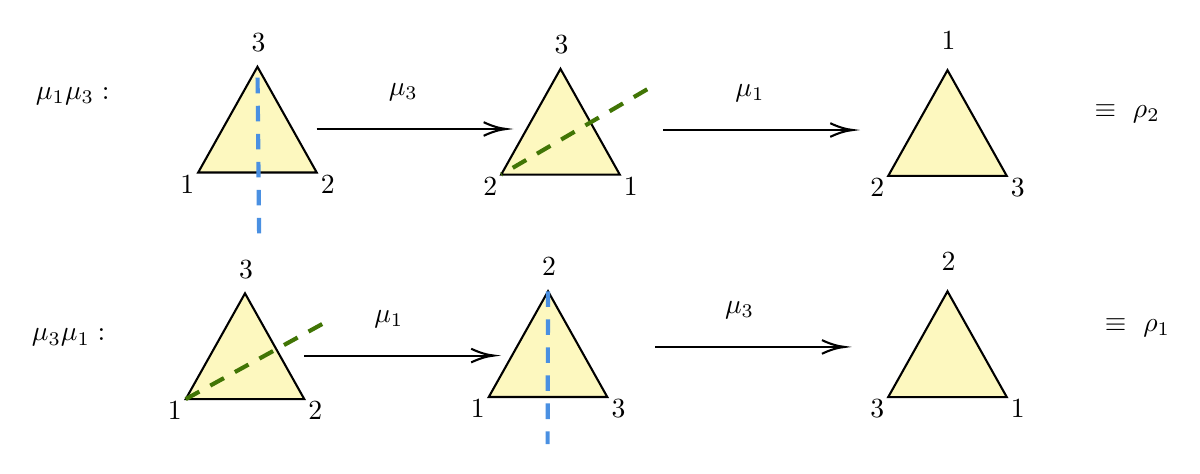
\begin{tikzpicture}[x=0.75pt,y=0.75pt,yscale=-1,xscale=1]
%uncomment if require: \path (0,213); %set diagram left start at 0, and has height of 213

%Straight Lines [id:da23227613985646378] 
\draw    (346.75,55.73) -- (436.12,55.73) ;
\draw [shift={(438.12,55.73)}, rotate = 180] [color={rgb, 255:red, 0; green, 0; blue, 0 }  ][line width=0.75]    (10.93,-3.29) .. controls (6.95,-1.4) and (3.31,-0.3) .. (0,0) .. controls (3.31,0.3) and (6.95,1.4) .. (10.93,3.29)   ;
%Straight Lines [id:da2537972233308252] 
\draw    (342.75,160.24) -- (432.12,160.24) ;
\draw [shift={(434.12,160.24)}, rotate = 180] [color={rgb, 255:red, 0; green, 0; blue, 0 }  ][line width=0.75]    (10.93,-3.29) .. controls (6.95,-1.4) and (3.31,-0.3) .. (0,0) .. controls (3.31,0.3) and (6.95,1.4) .. (10.93,3.29)   ;
%Shape: Triangle [id:dp5138384240785593] 
\draw  [fill={rgb, 255:red, 250; green, 238; blue, 106 }  ,fill opacity=0.43 ] (483.67,26.9) -- (512.22,77.84) -- (455.11,77.84) -- cycle ;
%Shape: Triangle [id:dp9299490724469842] 
\draw  [fill={rgb, 255:red, 250; green, 238; blue, 106 }  ,fill opacity=0.43 ] (483.67,133.45) -- (512.22,184.39) -- (455.11,184.39) -- cycle ;
%Shape: Triangle [id:dp3094198210232113] 
\draw  [fill={rgb, 255:red, 250; green, 238; blue, 106 }  ,fill opacity=0.43 ] (291.21,133.43) -- (319.76,184.37) -- (262.65,184.37) -- cycle ;

%Shape: Triangle [id:dp6072285341774635] 
\draw  [fill={rgb, 255:red, 250; green, 238; blue, 106 }  ,fill opacity=0.43 ] (145.21,134.43) -- (173.76,185.37) -- (116.65,185.37) -- cycle ;

%Straight Lines [id:da9916566252372986] 
\draw    (173.75,164.4) -- (263.12,164.4) ;
\draw [shift={(265.12,164.4)}, rotate = 180] [color={rgb, 255:red, 0; green, 0; blue, 0 }  ][line width=0.75]    (10.93,-3.29) .. controls (6.95,-1.4) and (3.31,-0.3) .. (0,0) .. controls (3.31,0.3) and (6.95,1.4) .. (10.93,3.29)   ;
%Straight Lines [id:da3884795444667827] 
\draw [color={rgb, 255:red, 65; green, 117; blue, 5 }  ,draw opacity=1 ][line width=1.5]  [dash pattern={on 5.63pt off 4.5pt}]  (116.65,185.37) -- (183,148.88) ;
%Shape: Triangle [id:dp4067226035070607] 
\draw  [fill={rgb, 255:red, 250; green, 238; blue, 106 }  ,fill opacity=0.43 ] (297.21,26.26) -- (325.76,77.2) -- (268.65,77.2) -- cycle ;

%Shape: Triangle [id:dp737332924910008] 
\draw  [fill={rgb, 255:red, 250; green, 238; blue, 106 }  ,fill opacity=0.43 ] (151.21,25.26) -- (179.76,76.2) -- (122.65,76.2) -- cycle ;

%Straight Lines [id:da7337740639590441] 
\draw    (179.75,55.24) -- (269.12,55.24) ;
\draw [shift={(271.12,55.24)}, rotate = 180] [color={rgb, 255:red, 0; green, 0; blue, 0 }  ][line width=0.75]    (10.93,-3.29) .. controls (6.95,-1.4) and (3.31,-0.3) .. (0,0) .. controls (3.31,0.3) and (6.95,1.4) .. (10.93,3.29)   ;
%Straight Lines [id:da9237438755224345] 
\draw [color={rgb, 255:red, 74; green, 144; blue, 226 }  ,draw opacity=1 ][line width=1.5]  [dash pattern={on 5.63pt off 4.5pt}]  (152,105.57) -- (151.21,25.26) ;
%Straight Lines [id:da1778028966163362] 
\draw [color={rgb, 255:red, 74; green, 144; blue, 226 }  ,draw opacity=1 ][line width=1.5]  [dash pattern={on 5.63pt off 4.5pt}]  (291.21,133.43) -- (291,207.1) ;
%Straight Lines [id:da5297072499212381] 
\draw [color={rgb, 255:red, 65; green, 117; blue, 5 }  ,draw opacity=1 ][line width=1.5]  [dash pattern={on 5.63pt off 4.5pt}]  (339,36.1) -- (268.65,77.2) ;

% Text Node
\draw (41,150.12) node [anchor=north west][inner sep=0.75pt]    {$\mu _{3} \mu _{1} :$};
% Text Node
\draw (43,33.63) node [anchor=north west][inner sep=0.75pt]    {$\mu _{1} \mu _{3} :$};
% Text Node
\draw (380,32.4) node [anchor=north west][inner sep=0.75pt]    {$\mu _{1}$};
% Text Node
\draw (375,136.91) node [anchor=north west][inner sep=0.75pt]    {$\mu _{3}$};
% Text Node
\draw (445.03,77.64) node [anchor=north west][inner sep=0.75pt]    {$2$};
% Text Node
\draw (512.75,77.64) node [anchor=north west][inner sep=0.75pt]    {$3$};
% Text Node
\draw (479.3,6.92) node [anchor=north west][inner sep=0.75pt]    {$1$};
% Text Node
\draw (445.03,184.19) node [anchor=north west][inner sep=0.75pt]    {$3$};
% Text Node
\draw (512.75,184.19) node [anchor=north west][inner sep=0.75pt]    {$1$};
% Text Node
\draw (479.3,113.47) node [anchor=north west][inner sep=0.75pt]    {$2$};
% Text Node
\draw (206,141.08) node [anchor=north west][inner sep=0.75pt]    {$\mu _{1}$};
% Text Node
\draw (213,31.91) node [anchor=north west][inner sep=0.75pt]    {$\mu _{3}$};
% Text Node
\draw (553,41.97) node [anchor=north west][inner sep=0.75pt]    {$\equiv \ \rho _{2}$};
% Text Node
\draw (558,144.97) node [anchor=north west][inner sep=0.75pt]    {$\equiv \ \rho _{1}$};
% Text Node
\draw (146.84,7.8) node [anchor=north west][inner sep=0.75pt]    {$3$};
% Text Node
\draw (180.29,76) node [anchor=north west][inner sep=0.75pt]    {$2$};
% Text Node
\draw (112.57,76) node [anchor=north west][inner sep=0.75pt]    {$1$};
% Text Node
\draw (292.84,8.8) node [anchor=north west][inner sep=0.75pt]    {$3$};
% Text Node
\draw (326.29,77) node [anchor=north west][inner sep=0.75pt]    {$1$};
% Text Node
\draw (258.57,77) node [anchor=north west][inner sep=0.75pt]    {$2$};
% Text Node
\draw (140.84,116.97) node [anchor=north west][inner sep=0.75pt]    {$3$};
% Text Node
\draw (174.29,185.17) node [anchor=north west][inner sep=0.75pt]    {$2$};
% Text Node
\draw (106.57,185.17) node [anchor=north west][inner sep=0.75pt]    {$1$};
% Text Node
\draw (286.84,115.97) node [anchor=north west][inner sep=0.75pt]    {$2$};
% Text Node
\draw (320.29,184.17) node [anchor=north west][inner sep=0.75pt]    {$3$};
% Text Node
\draw (252.57,184.17) node [anchor=north west][inner sep=0.75pt]    {$1$};


\end{tikzpicture}
